\documentclass[11pt,a4paper]{article}

\usepackage[utf8]{inputenc}
\usepackage[T1]{fontenc}
\usepackage[brazil]{babel}
\usepackage{lmodern}
\usepackage{geometry}
\usepackage{graphicx}
\usepackage{booktabs}
\usepackage{float}
\usepackage{amsmath}
\usepackage{microtype}
\usepackage[authoryear]{natbib}
\usepackage[colorlinks=true,linkcolor=black,citecolor=black,urlcolor=blue]{hyperref}

\geometry{margin=2.5cm}
\graphicspath{{../../figures/}}
\setlength{\parskip}{0.6em}
\setlength{\parindent}{0pt}

\title{LLMs sob o Microscópio:\\Incerteza, Poder Estatístico e a Ilusão do Ranking Exato}
\author{Diego Henrique Xavier}
\date{2026}

\begin{document}

\maketitle

\begin{abstract}
Rankings públicos de modelos de linguagem costumam tratar diferenças de décimos de ponto percentual como fatos precisos. Este projeto reexamina essa leitura ao tratar scores de benchmark como estimativas com amostra finita, e não como medidas exatas. Usando 4.496 modelos do Open LLM Leaderboard v2 e cerca de 33 mil batalhas do LMSYS Chatbot Arena, a análise aplica intervalos de Wilson, bootstrap não paramétrico, testes pareados com correção de Benjamini--Hochberg, análise de poder estatístico, modelagem Bradley--Terry e comparações em escala Elo. Os resultados mostram que a margem de erro teórica do GPQA supera \(\pm 4{,}6\) pontos percentuais perto de \(p=0{,}5\), que mais de 60\% dos pares do top-100 nesse benchmark são estatisticamente indistinguíveis e que a correção para múltiplas comparações reduz fortemente a fração de diferenças significativas no topo. Metadados sozinhos explicam cerca de \(R^2 \approx 0{,}70\) do average via XGBoost, enquanto a Arena concorda qualitativamente com a ordenação do leaderboard nos modelos em comum. A implicação central é prática: posição exata costuma ser artefato de relato, e a escolha de modelo deve ser feita por tier estatístico.
\end{abstract}

\textbf{Palavras-chave:} modelos de linguagem; benchmarks; inferência binomial; bootstrap; Bradley--Terry; Chatbot Arena.

\section{Introdução}
Rankings de LLMs são frequentemente lidos como se a posição 1 fosse claramente diferente da posição 5, mesmo quando a distância é de frações de ponto percentual. Essa interpretação é fraca quando cada score é apenas uma estimativa calculada sobre um conjunto finito de questões. Se um benchmark contém \(n\) itens, o score observado é uma proporção binomial sujeita a variabilidade amostral. Quando a incerteza é explicitada, boa parte das diferenças finas deixa de sustentar uma leitura determinística.

Este estudo responde a uma pergunta direta: quanto do que é publicado como ranking resiste a uma análise estatística convencional? A resposta importa porque leaderboards públicos já influenciam decisões de produto, narrativa de pesquisa e alegações sobre progresso em modelos.

Os objetivos do projeto são quatro:
\begin{enumerate}
    \item quantificar a incerteza dos benchmarks públicos com estimativas intervalares;
    \item testar se modelos adjacentes no topo permanecem separáveis após correção de múltiplas comparações;
    \item avaliar se o tamanho atual dos benchmarks tem poder suficiente para sustentar alegações finas de ranking;
    \item comparar a ordenação de benchmark com dados de preferência humana da Arena.
\end{enumerate}

\section{Referencial Teórico}
O núcleo estatístico do problema é simples. A acurácia em benchmark pode ser escrita como \(\hat{p}=k/n\), em que \(k\) é o número de acertos em \(n\) questões. Para intervalos de confiança, este trabalho usa o intervalo score de Wilson \citep{wilson1927}, que costuma ter comportamento melhor que o intervalo de Wald, sobretudo longe do centro e com tamanho amostral moderado \citep{agresti1998}. Para visualização do topo e comunicação, também se usa bootstrap não paramétrico \citep{efron1979}.

Comparações pareadas criam um segundo problema. Um top-50 implica \(50\times49/2 = 1{,}225\) testes simultâneos. Sem correção, muitas diferenças aparentemente significativas surgem por acaso. Para enfrentar isso, a análise controla a false discovery rate com o procedimento de Benjamini--Hochberg \citep{benjamini1995}. O tamanho de efeito é reportado com o \(h\) de Cohen para proporções \citep{cohen1988}.

Nas batalhas da Arena, o ranking é modelado com Bradley--Terry \citep{bradley1952} estimado pelo algoritmo MM de \citet{ford1957}. As forças também são lidas em escala Elo por conveniência interpretativa \citep{elo1978}. O leaderboard e a Arena são complementares: o primeiro depende de benchmarks estruturados, enquanto a segunda depende de comparações cegas por preferência humana \citep{zheng2023arena,arena2026}.

\section{Dados e Métodos}

\subsection{Bases de dados}
O lado de benchmark usa o Open LLM Leaderboard v2 \citep{huggingface2024leaderboard}, após remover entradas sinalizadas pelos próprios mantenedores. A base analítica final contém 4.496 modelos e seis benchmarks centrais: IFEval, BBH, MATH Lvl 5, GPQA, MuSR e MMLU-PRO. Metadados como escala de parâmetros, família arquitetural, precisão e organização foram extraídos dos identificadores publicados.

O lado de preferência usa cerca de 33 mil batalhas do ecossistema LMSYS Chatbot Arena \citep{zheng2023arena,arena2026}. Empates foram removidos do ajuste principal de Bradley--Terry para que cada batalha retida representasse uma comparação decisiva.

\subsection{Pipeline estatístico}
O código do repositório foi organizado em dez etapas sequenciais: ingestão, pré-processamento, auditoria, análise exploratória, inferência, aprendizado de máquina, ranking, modelagem da Arena e consolidação final. Os principais parâmetros foram:
\begin{itemize}
    \item intervalos de Wilson a 95\%;
    \item bootstrap com 2.000 reamostragens para os gráficos de ranking;
    \item correção de Benjamini--Hochberg com \(\alpha = 0{,}05\);
    \item análise de poder com \(\alpha = 0{,}05\) e poder \(= 0{,}80\);
    \item ajuste Bradley--Terry com intervalos bootstrap na fatia da Arena.
\end{itemize}

\subsection{Quantidades derivadas}
Três quantidades sintetizam a leitura:
\begin{enumerate}
    \item a margem de erro teórica implicada por cada benchmark;
    \item a fração de pares no topo cuja diferença é pequena demais para ser distinguida;
    \item o número de itens que seria necessário para separar com confiança modelos do topo quando a diferença observada é usada como tamanho de efeito.
\end{enumerate}

\section{Resultados}

\subsection{O tamanho do benchmark governa a incerteza}
O primeiro resultado é mecânico, mas decisivo. O comprimento do benchmark não é detalhe lateral; ele define a precisão do ranking. O GPQA, com apenas 448 questões, implica uma faixa de incerteza muito maior que o MMLU-PRO, que possui 12.032 itens.

\begin{table}[H]
\centering
\caption{Tamanho do benchmark e margem de erro teórica de Wilson em \(p=0{,}5\)}
\begin{tabular}{lrr}
\toprule
Benchmark & \(n\) & MOE (pp) \\
\midrule
GPQA & 448 & 4,6 \\
IFEval & 541 & 4,2 \\
MuSR & 756 & 3,6 \\
MATH Lvl 5 & 1.324 & 2,7 \\
BBH & 6.511 & 1,2 \\
MMLU-PRO & 12.032 & 0,9 \\
\bottomrule
\end{tabular}
\end{table}

\begin{figure}[H]
\centering
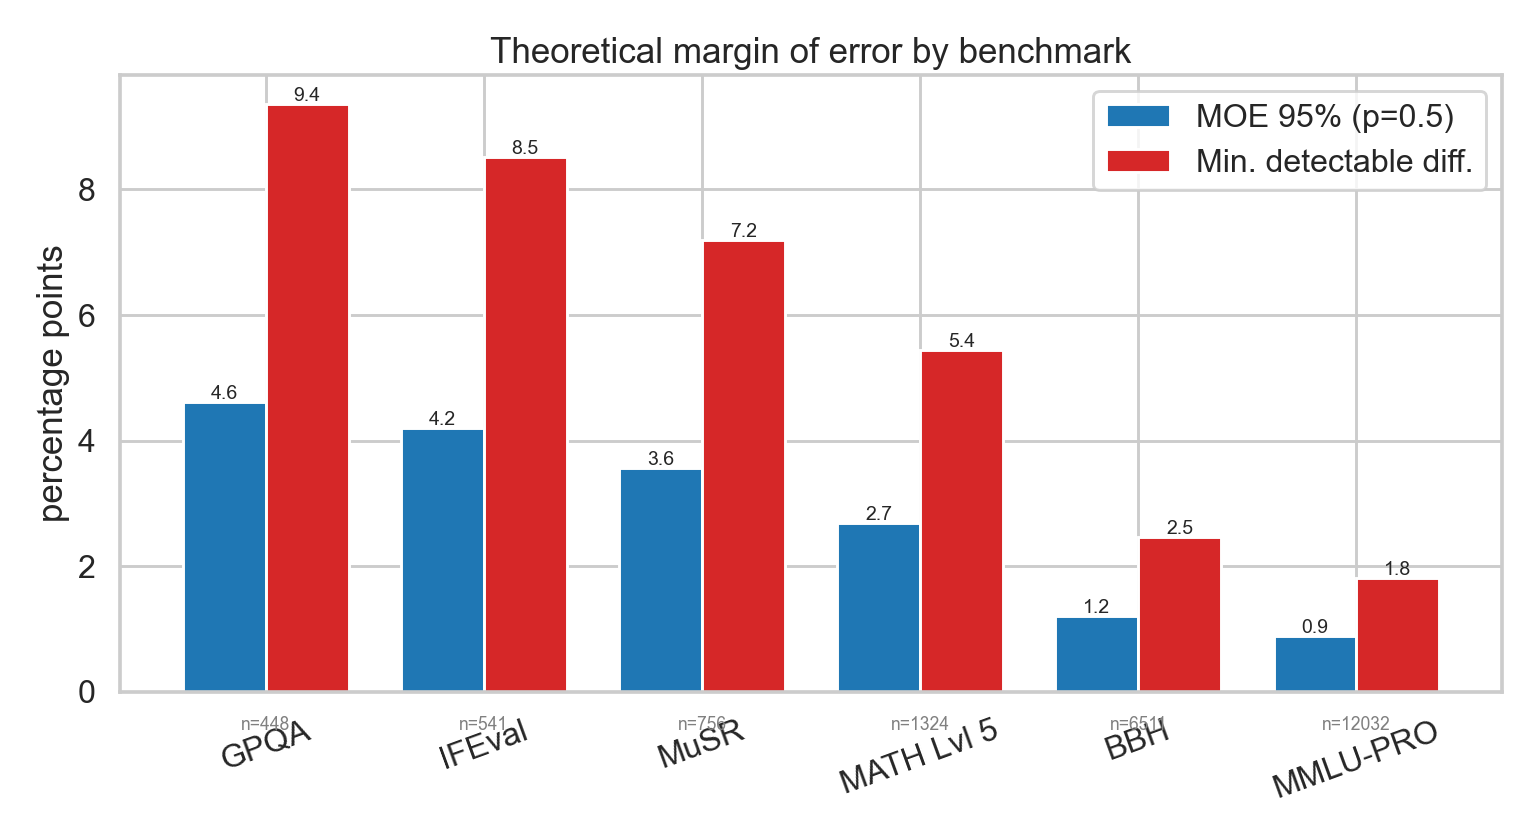
\includegraphics[width=0.8\textwidth]{04_moe_teorica.png}
\caption{Margem de erro teórica por benchmark.}
\end{figure}

Essa diferença de escala muda o significado do ranking. No GPQA, um gap de três pontos pode ser menor que a própria incerteza de cada estimativa. No MMLU-PRO, o mesmo gap é bem mais defensável.

\subsection{Grande parte dos pares do topo não é claramente separável}
O projeto estima quantos pares do top-100 têm diferenças menores que a diferença mínima detectável implicada pelo tamanho do benchmark. GPQA e MuSR são os alertas mais fortes: a maior parte dos gaps pareados no topo é pequena demais para sustentar uma leitura determinística.

\begin{figure}[H]
\centering
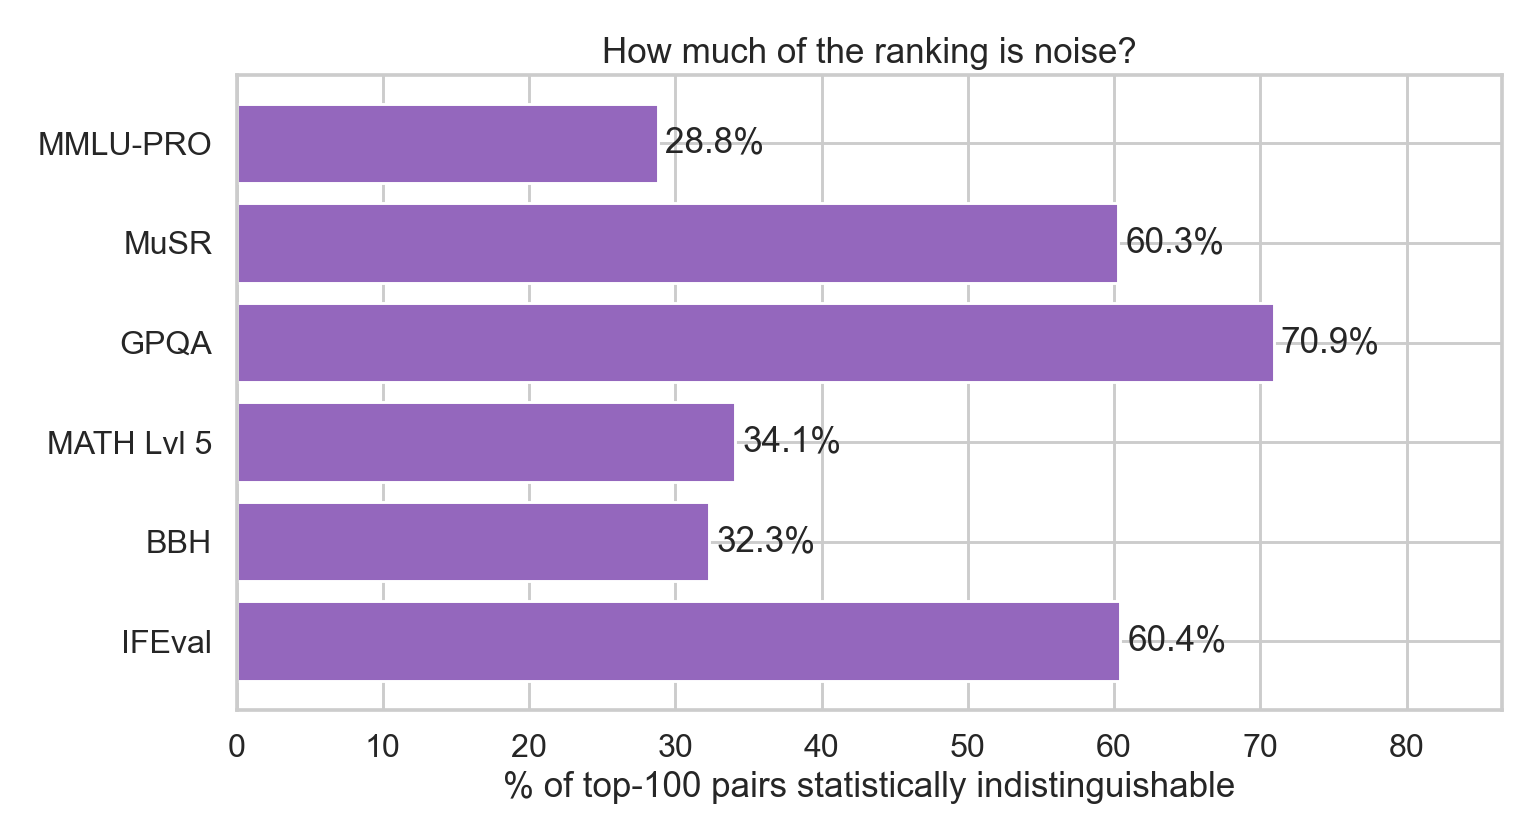
\includegraphics[width=0.8\textwidth]{04_pct_pares_indistinguiveis.png}
\caption{Fração de pares estatisticamente indistinguíveis no top-100.}
\end{figure}

A leitura prática é direta. Um leaderboard pode listar um modelo acima de outro, mas o \(n\) disponível muitas vezes não sustenta a afirmação de que o modelo superior é realmente melhor e não apenas um pouco à frente em uma estimativa ruidosa.

\subsection{A correção de múltiplas comparações remove boa parte da significância aparente}
Testes pareados brutos no top-50 geram mais de mil comparações por benchmark. Após controle da false discovery rate, a fração de pares significativos cai materialmente, sobretudo nos benchmarks menores.

\begin{figure}[H]
\centering
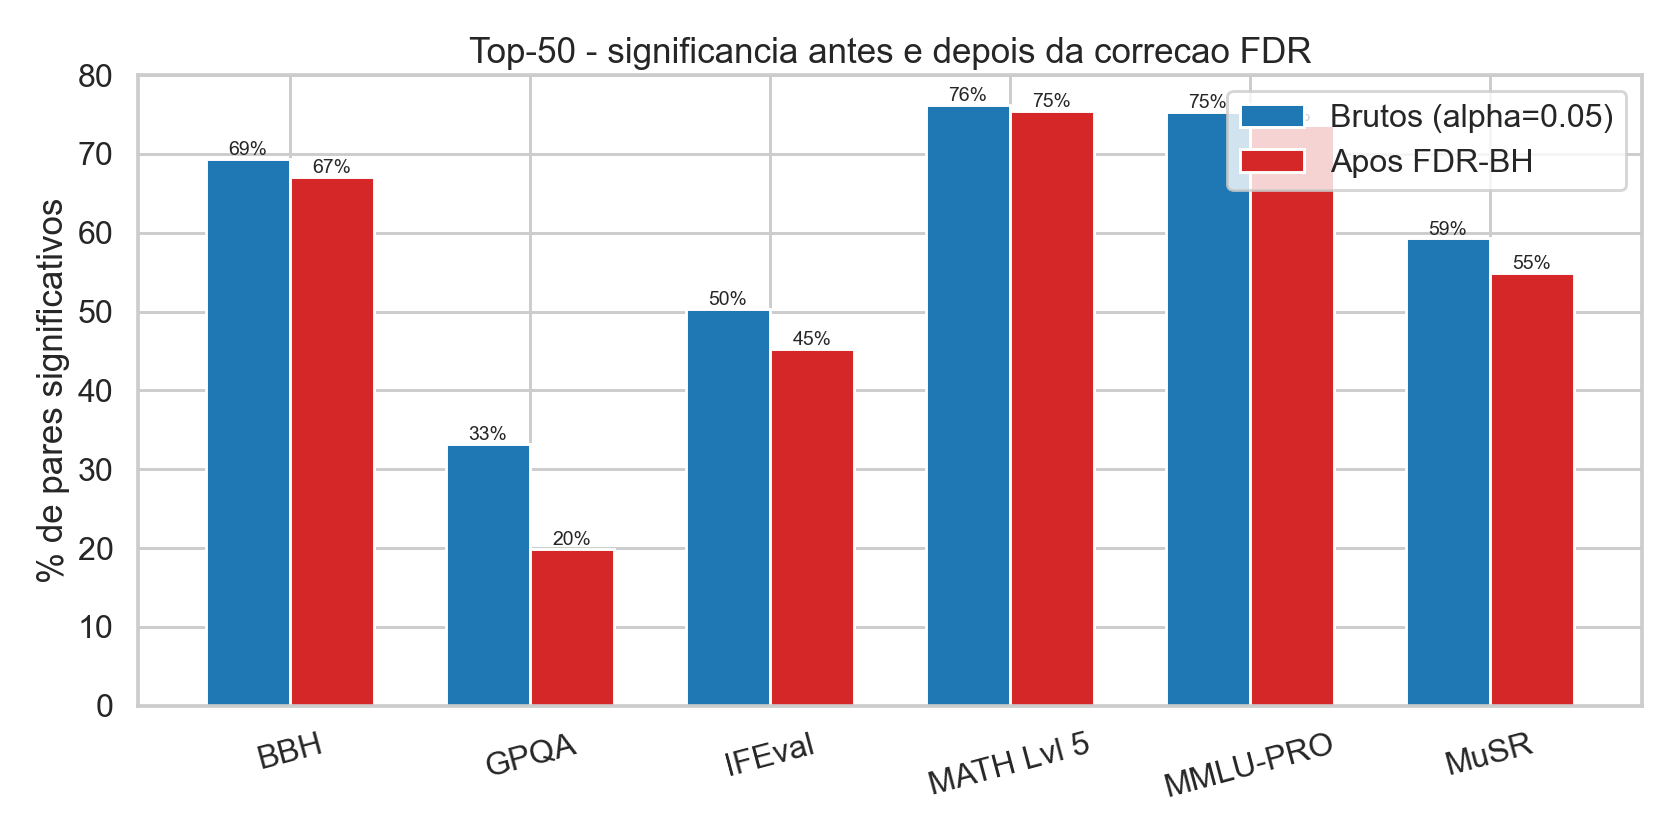
\includegraphics[width=0.8\textwidth]{06_pct_significativos_fdr.png}
\caption{Significância pareada no top-50 antes e depois da correção de Benjamini--Hochberg.}
\end{figure}

O efeito é mais forte no GPQA, em que a fração ajustada de pares significativos se torna pequena. Esse padrão é exatamente o esperado quando muitas descobertas brutas são infladas pela multiplicidade, e não por separação robusta.

\subsection{O poder atual costuma ser insuficiente para ranking fino}
Usando a diferença observada entre top-1 e top-10 como tamanho de efeito alvo, a análise de poder mostra que vários benchmarks precisariam de muito mais itens para sustentar distinções finas no topo.

\begin{table}[H]
\centering
\caption{Análise de poder para separar top-1 de top-10}
\begin{tabular}{lrr}
\toprule
Benchmark & \(n\) atual & \(n\) necessário para 80\% de poder \\
\midrule
GPQA & 448 & \(> 5.000\) \\
IFEval & 541 & \(> 3.000\) \\
MuSR & 756 & \(> 4.000\) \\
MATH Lvl 5 & 1.324 & \(\approx 900\) \\
BBH & 6.511 & \(\approx 500\) \\
MMLU-PRO & 12.032 & \(\approx 300\) \\
\bottomrule
\end{tabular}
\end{table}

Isso ajuda a explicar por que tantas posições vizinhas se sobrepõem. O problema não é apenas a incerteza de um score isolado. Também há falta de poder para a própria pergunta de ranking que o público quer responder.

\subsection{Bootstrap favorece tiers em vez de posições exatas}
O bootstrap de posição torna a sobreposição explícita. Mesmo ordenando os modelos pela mediana da posição, os intervalos de 95\% frequentemente cobrem muitas colocações.

\begin{figure}[H]
\centering
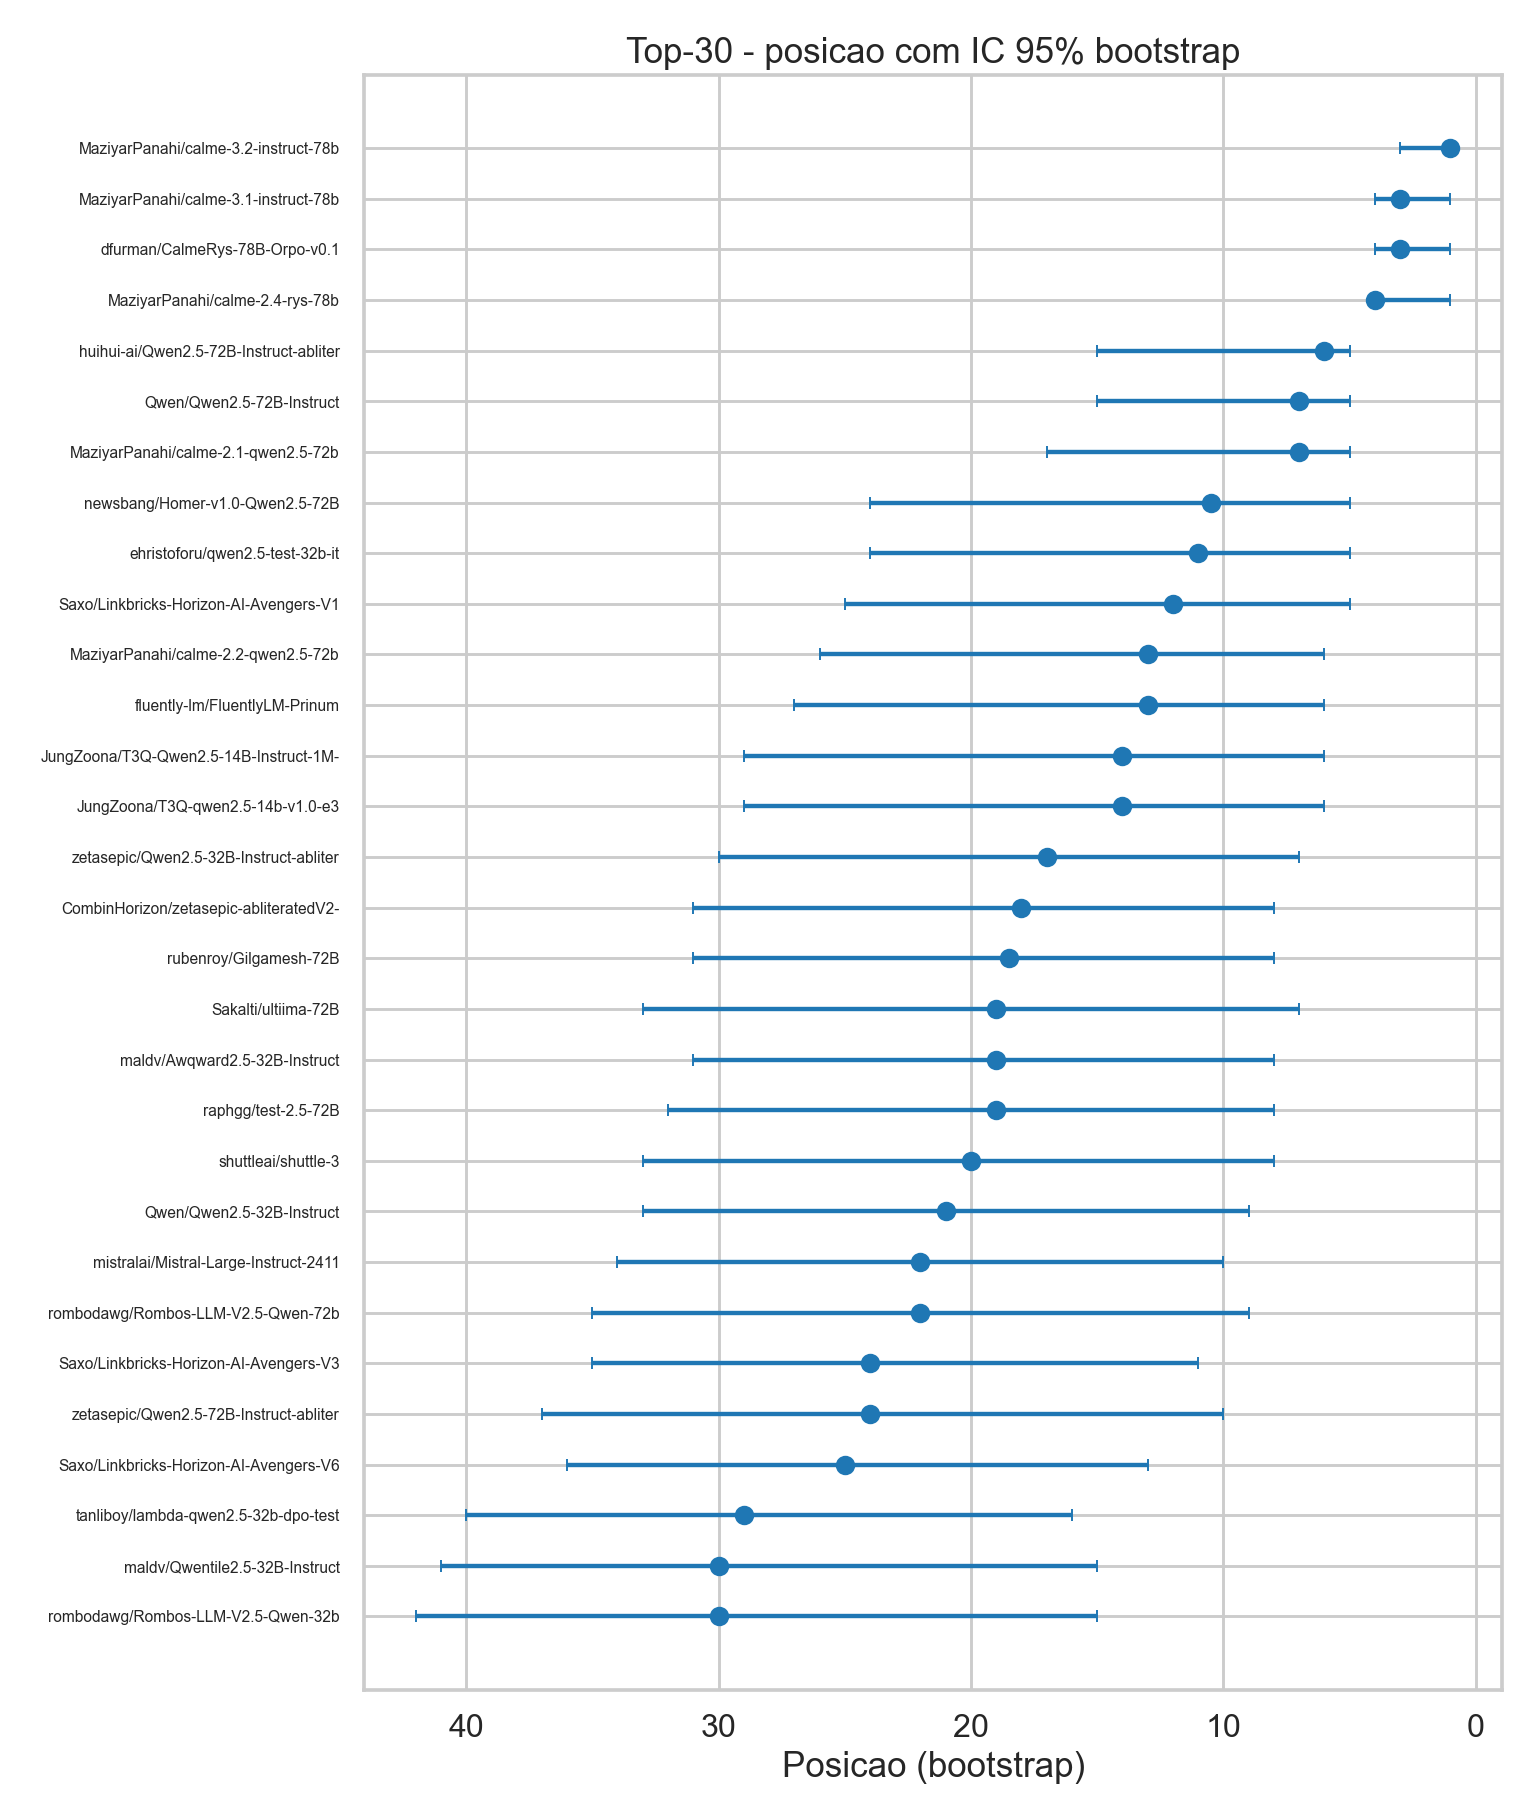
\includegraphics[width=\textwidth]{08_ranking_bootstrap_top30.png}
\caption{Top-30 com posição mediana bootstrap e intervalo de 95\%.}
\end{figure}

O ranking, portanto, é melhor resumido como um conjunto pequeno de tiers estatísticos, e não como dezenas de posições exatas defendáveis.

\subsection{Metadados explicam a maior parte da ordenação visível}
Um experimento separado de aprendizado de máquina regressa o average do leaderboard apenas com metadados. O melhor modelo, XGBoost, alcança cerca de \(R^2 = 0{,}70\) em dados fora da amostra. Isso significa que grande parte da ordenação visível já é capturada por variáveis como escala de parâmetros, família arquitetural, precisão e organização.

\begin{figure}[H]
\centering
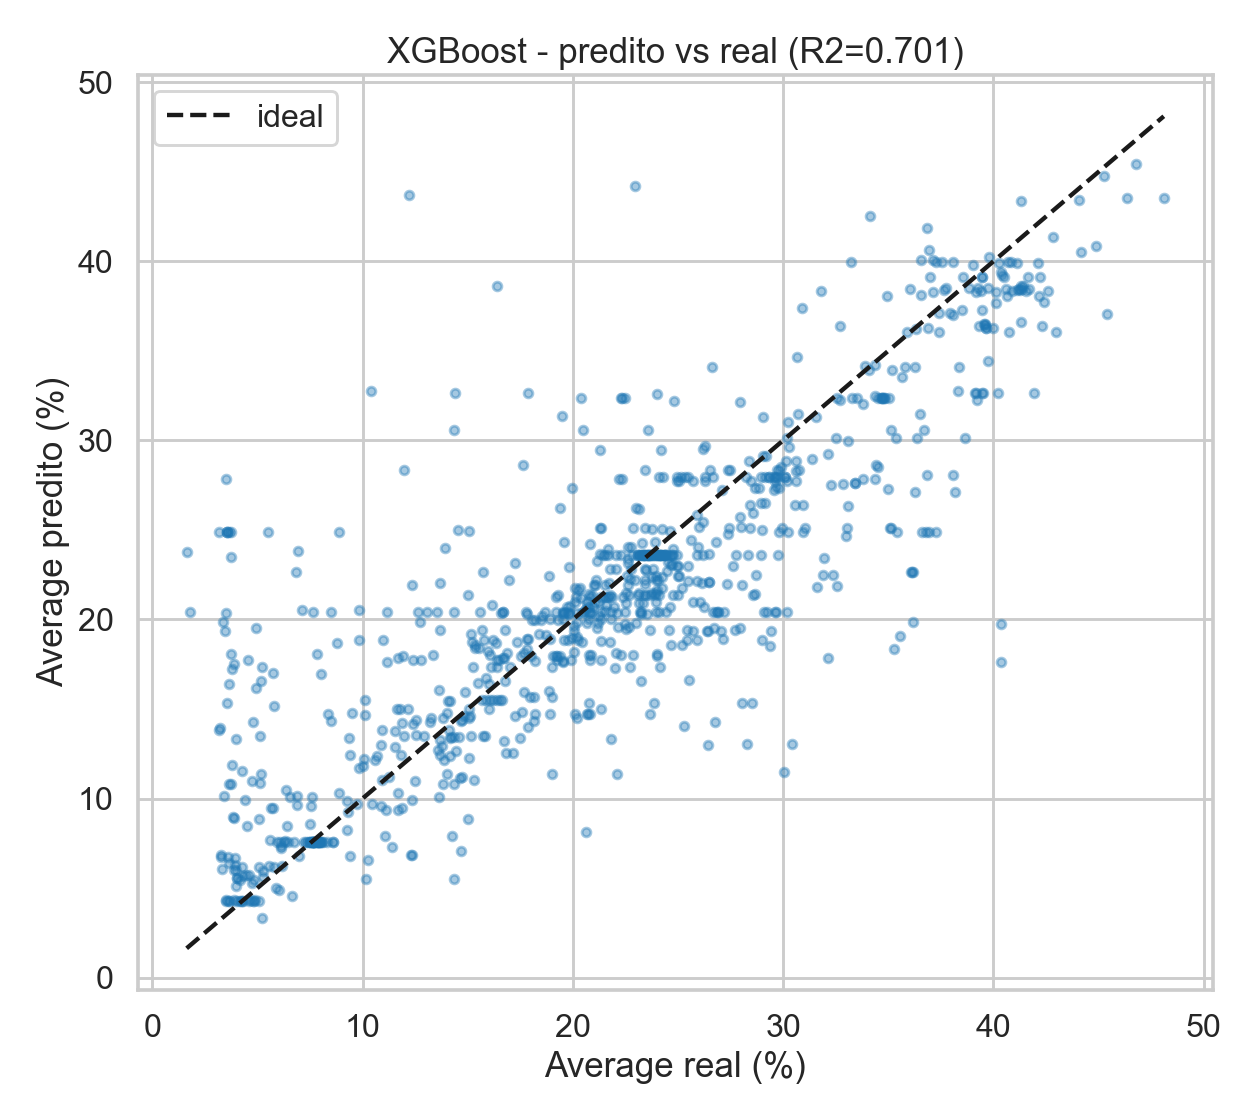
\includegraphics[width=0.78\textwidth]{07_pred_vs_real_xgb.png}
\caption{Average do leaderboard previsto apenas com metadados.}
\end{figure}

Esse resultado não implica que detalhes de arquitetura e treinamento não importam. Ele implica que grande parte da variação observada no topo deixa de ser surpreendente quando se conhece a estrutura grosseira do modelo. O resíduo é onde as inovações reais tendem a aparecer.

\subsection{A Arena conta a mesma história geral}
As batalhas de preferência da Arena foram modeladas com Bradley--Terry e reportadas em escala Elo. O topo da Arena se organiza em um tier superior mais nítido, mas a maior parte dos modelos vizinhos ainda apresenta sobreposição nos intervalos de incerteza.

\begin{figure}[H]
\centering
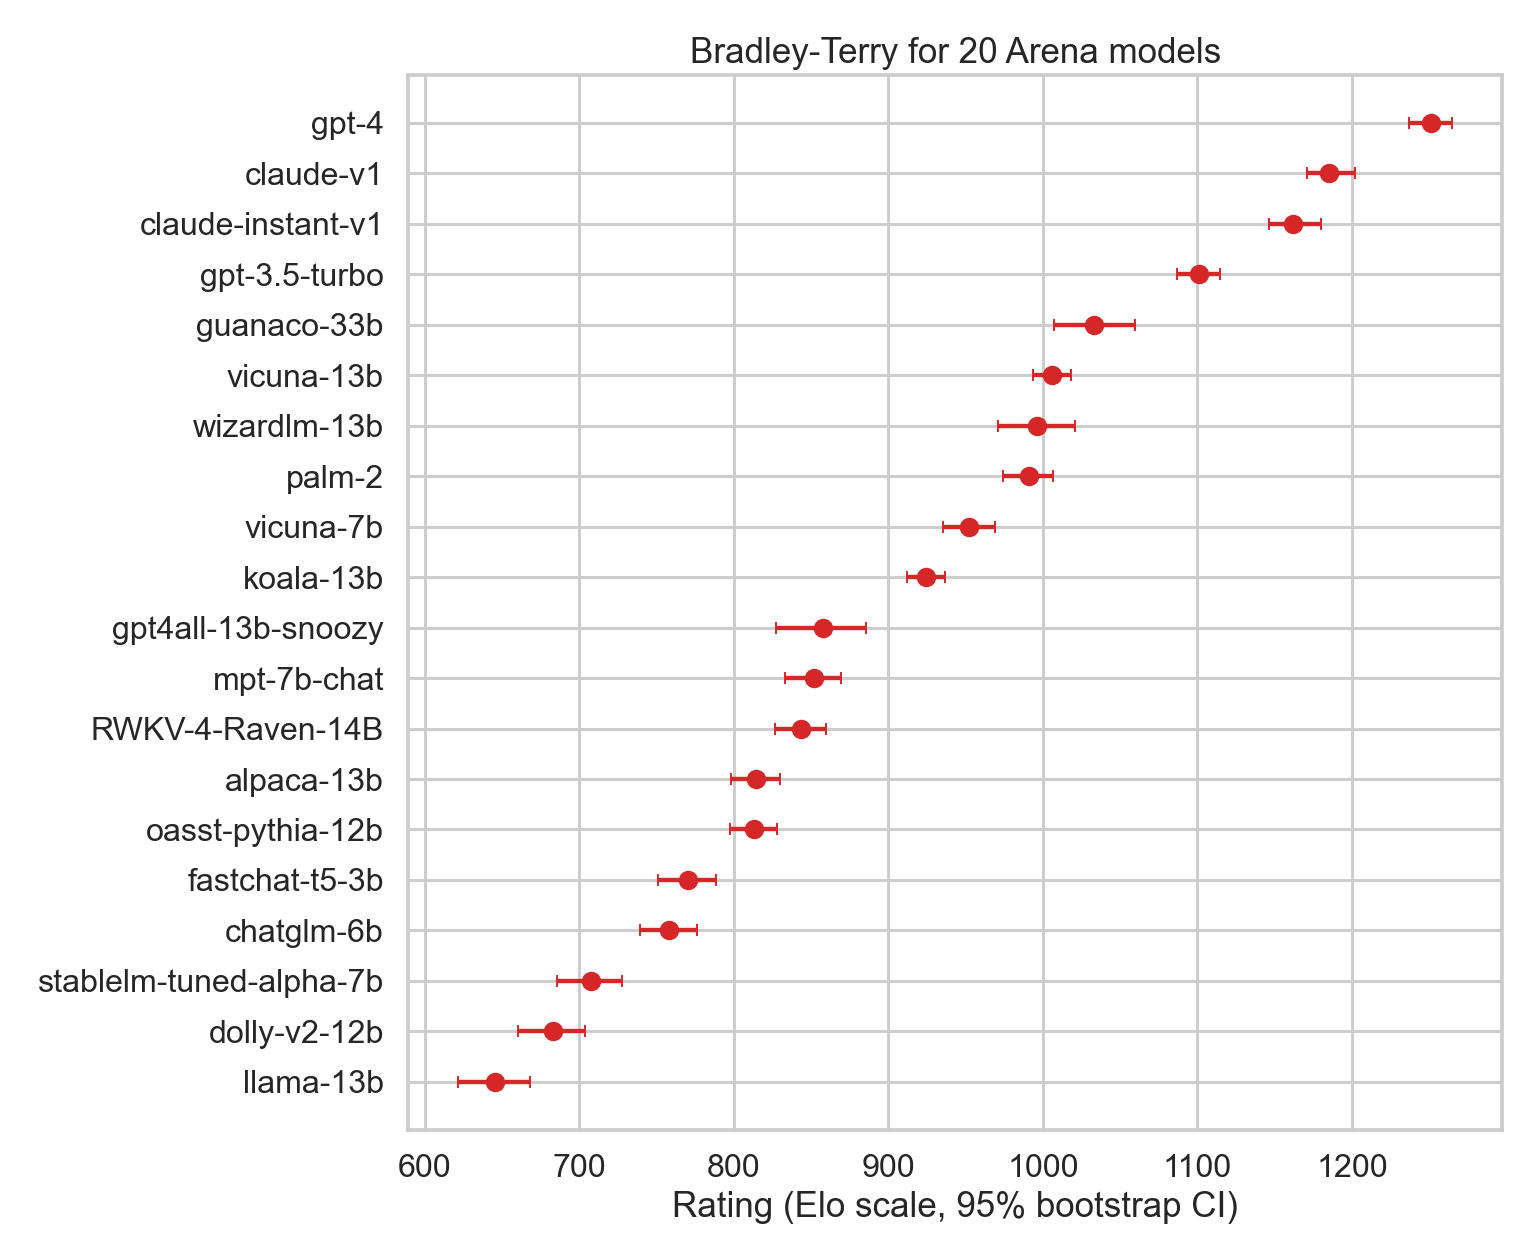
\includegraphics[width=0.82\textwidth]{09_bradley_terry.png}
\caption{Ajuste Bradley--Terry da Arena em escala Elo com intervalos bootstrap.}
\end{figure}

Nos modelos compartilhados entre as duas bases, a ordenação qualitativa é preservada. A interseção é pequena, mas informativa: diferenças grandes parecem reais em regimes de avaliação distintos, enquanto microdiferenças seguem frágeis.

\section{Discussão}
Três conclusões se destacam.

Primeiro, a incerteza não é enfeite. Ela muda a interpretação do leaderboard. Em benchmarks curtos, o intervalo de confiança já é suficiente para impedir que modelos consecutivos no topo sejam distinguidos com honestidade estatística.

Segundo, o problema é agravado pela multiplicidade. Quando o número de testes pareados é explicitado e a FDR é controlada, boa parte da significância aparente desaparece. Isso significa que a linguagem de ranking exato costuma ser mais forte do que o dado sustenta.

Terceiro, a unidade mais defensável de decisão é o tier, e não a posição. A combinação de intervalos largos, baixo poder para comparações topo-contra-topo e sobreposição no bootstrap leva à mesma recomendação operacional: tratar o topo do leaderboard como grupos amplos e incertos, e não como uma ordem precisa.

\section{Conclusão}
Este projeto entrega uma releitura estatística completa de rankings públicos de LLMs. Ao combinar incerteza de benchmark, inferência pareada, análise de poder, modelagem por metadados e comparação com a Arena, a evidência converge para a mesma direção: a posição exata no leaderboard muitas vezes é mais artefato de precisão de relato do que fato empírico estável.

Para a prática de avaliação, a implicação é simples e importante. Leaderboards públicos continuam úteis, mas devem ser lidos como instrumentos comparativos ruidosos. Quando as diferenças são pequenas, rank precisa ser convertido em tiers com incerteza explícita antes de orientar produto, pesquisa ou comunicação.

\bibliographystyle{plainnat}
\bibliography{../references}

\end{document}
